% !TeX root = RJwrapper.tex
\title{Explaining Predictions with Shapley Values in R}
\author{by Brandon M. Greenwell}

\maketitle

\abstract{%
An abstract of less than 150 words.
}

\hypertarget{introduction}{%
\section{Introduction}\label{introduction}}

The \emph{Shapley value} (Shapley 2016) is an idea from coalitional/cooperative game theory. In a coalitional game (i.e., a competetive game between groups of players called \emph{coalitions}), assume we have \(p\) players that form a grand coalition (\(S\)) worth a certain payout (\(\Delta_S\)). Suppose we also know how much any smaller coalition (\(Q \subseteq S\)) (i.e., any subset of \(p\) players) is worth (\(\Delta_Q\)). The goal is to distribute the total payout \(\Delta_S\) to the individual \(p\) players in a ``fair'' way; that is, so that each player receives their ``fair'' share. The Shapley value is one such solution and the only one that uniquely satisfies a particular set of ``fairness properties.''

Let \(v\) be a \emph{characteristic function} (or mapping) that assigns a value to each subset of players; in particular, \(v : 2^p \rightarrow \mathbb{R}\), where \(v\left(S\right) = \Delta_S\), \(v\left(\emptyset\right) = 0\), and \(\emptyset\) is the empty set (i.e., zero players). Let \(\phi_i\left(v\right)\) be the contribution (or portion of the total payout) attributed to player \(i\) in a particular game with total payout \(v\left(S\right) = \Delta_S\). The Shapley values \(\left\{\phi_i\right\}_{i=1}^p\) satisfy the following four properties:

\begin{enumerate}
\def\labelenumi{\arabic{enumi}.}
\item
  Efficiency: \(\sum_{i = 1} ^ p \phi_i\left(v\right) = \Delta_S\).
\item
  Null player: \(\forall W \subseteq S \setminus \left\{i\right\}: \Delta_W = \Delta_{W \cup \left\{i\right\}} \implies \phi_i\left(v\right) = 0\).
\item
  Symmetry: \(\forall W \subseteq S \setminus \left\{i, j\right\}: \Delta_{W \cup \left\{i\right\}} = \Delta_{W \cup \left\{j\right\}} \implies \phi_i\left(v\right) = \phi_j\left(v\right)\).
\item
  Linearity: If \(v\) and \(w\) are functions describing two coalitional games, then \(\phi_i\left(v + w\right) = \phi_i\left(v\right) + \phi_i\left(w\right)\).
\end{enumerate}

The above properties can be interpreted as follows: 1) the individual player contributions sum to the total payout, hence, are implicitly normalized; 2) if a player does not contribute to any coalition they receive a payout of zero; 3) if two players have the same impact across all coalitions, they receive equal payout; and 4) the local contributions are additive across different games.

Shapley (2016) showed that the unique solution satisfying the above properties is given by

\begin{equation}
\phi_i\left(x\right) = \frac{1}{p!} \sum_{\mathcal{O} \in \pi\left(p\right)} \left[v\left(S^\mathcal{O} \cup i\right) - v\left(S^\mathcal{O}\right)\right], \quad i = 1, 2, \dots, p,
  \label{eq:shapley-value}
\end{equation}
where \(\mathcal{O}\) is a specific permutation of the players indices \(\left\{1, 2, \dots, p\right\}\), \(\pi\left(p\right)\) is the set of all such permutations of size \(p\), and \(S^\mathcal{O}\) is the set of players joining the coalition before player \(i\).

In other words, the Shapley value is the average marginal contribution of a player across all possible coalitions in a game. Another way to interpret Equation \eqref{eq:shapley-value} is as follows. Imagine the coalitions (i.e., subsets of players) being formed one player at a time (which can happen in different orders), with the \(i\)-th player demanding a fair contribution/payout of \(v\left(S^\mathcal{O} \cup i\right) - v\left(S^\mathcal{O}\right)\). The Shapley value for player \(i\) is given by the average of this contribution over all possible permutations in which the coalition can be formed.

A simple example may help clarify the main ideas. Suppose three friends (players)---Alex, Brad, and Brandon---decide to go out for drinks after work (the game). They shared a few pitchers of beer, but nobody payed attention to how much each person drank (collaborated). What's a fair way to split the tab (total payout)? Suppose we knew the follow information, perhaps based on historical data:

\begin{itemize}
\item
  If Alex drank alone, he'd only pay \$10.
\item
  If Brad drank alone, he'd only pay \$20.
\item
  If Brandon drank alone, he'd only pay \$10.
\item
  If Alex and Brad drank together, they'd only pay \$25.
\item
  If Alex and Brandon drank together, they'd only pay \$15.
\item
  If Brad and Brandon drank together, they'd only pay \$13.
\item
  If Alex, Brad, and Brandon drank together, they'd only pay \$30.
\end{itemize}

Note that \(S = \left\{\text{Alex}, \text{Brad}, \text{Brandon}\right\}\) and that \(\Delta_S = \$30\). With only three players, we can enumerate all possible coalitions. In Table \ref{tab:drinks-pdf}, we list out all possible permutations of the three players along with the marginal contribution of each. Take the first row, for example. In this particular permutation, we start with Alex. We know that if Alex drinks alone, he'd spend \$10, so his marginal contribution by entering first is \$10. Next, we assume Brad enters the coalition. We know that if Alex and Brad drank together, they'd pay a total of \$25, leaving \$15 left over for Brad's marginal contribution. Similarly, if Brandon joins the party last, his marginal contribution would be only \$5 (the difference between \$30 and \$25). The Shapley value for each player is the average marginal contribution across all six possible permutations (these are the column averages reported in the last row).

\begin{table}[!htb]

\caption{\label{tab:drinks-pdf}Marginal contribution for each permutation of the players {Alex, Brad, Brandon} (i.e., the order in which they arrive). The Shapley  contribution is the average marginal contribution cross all permutations. (Notice how each row sums to the total bill of \$30.)}
\centering
\begin{tabular}[t]{lrrr}
\toprule
Permutation/order of players & Alex & Brad & Brandon\\
\midrule
Alex, Brad, Brandon & \$10.00 & \$15.00 & \$5.00\\
Alex, Brandon, Brad & \$10.00 & \$15.00 & \$5.00\\
Brad, Alex, Brandon & \$5.00 & \$20.00 & \$5.00\\
Brad, Brandon, Alex & \$10.00 & \$20.00 & \$0.00\\
Brandon, Alex, Brad & \$5.00 & \$15.00 & \$10.00\\
Brandon, Brad, Alex & \$17.00 & \$3.00 & \$10.00\\
\midrule
Shapley contribution: & \$9.50 & \$14.67 & \$5.83\\
\bottomrule
\end{tabular}
\end{table}

In this example, Brandon would get away with the smallest payout (i.e., have to pay the smallest portion of the total tab). The next time the bartender asks how you want to split the tab, whip out a pencil and do the math! In the next section, we'll show how the same idea can be used to help quantify the contribution each feature value makes to its corresponding prediction in a machine learning model.

\hypertarget{shapley-values-for-explaining-predictions}{%
\section{Shapley values for explaining predictions}\label{shapley-values-for-explaining-predictions}}

Štrumbelj and Kononenko (2014) suggested using the Shapley value \eqref{eq:shapley-value} to help explain predictions from a machine learning model. In the context of machine learning:

\begin{itemize}
\item
  a game is represented by the prediction task for a single observation \(\boldsymbol{x} = \left(x_1, x_2, \dots, x_p\right)\) (i.e., there are \(p\) features in total);
\item
  the total payout/worth (\(\Delta_S\)) for \(\boldsymbol{x}\) is the prediction for \(\boldsymbol{x}\), denoted \(\hat{f}\left(\boldsymbol{x}\right)\), minus the average prediction for all training observations (call this the baseline prediction, which we'll denote by \(\bar{f}\));
\item
  the players are the individual feature values of \(\boldsymbol{x}\) that collaborate to receive the payout (i.e., \(\hat{f}\left(\boldsymbol{x}\right) - \bar{f}\)).
\end{itemize}

From the last point, it's important to note that Shapley explanations are not trying to quantify the contribution each feature value in \(\boldsymbol{x}\) makes to its prediction \(\hat{f}\left(\boldsymbol{x}\right)\), but rather to the quantity \(\hat{f}\left(\boldsymbol{x}\right) - \bar{f}\), the difference between its prediction and the baseline. This seems to be a common source of confusion in interpreting a set of Shapley explanations from a given model.

In the following sections, we'll discuss several popular ways to compute Shapley values in practice.

\hypertarget{choice-of-characteristic-function-v}{%
\subsection{\texorpdfstring{Choice of characteristic function \(v\)}{Choice of characteristic function v}}\label{choice-of-characteristic-function-v}}

The challenge of using Shapley values for the purpose of explaining predictions is in defining the functional form of \(v\). As discussed in H. Chen et al. (2020), there are several ways to do this. However, since we are primarily interested in understanding how much each feature contributed to a particular prediction, \(v\) is typically related to a conditional expectation of the model's prediction. H. Chen et al. (2020) make the distinction between two possibilities, each of which differs in their conditioning argument. The Shapley value implementations discussed in this paper (e.g., MC SHAP and Tree SHAP) rely on what H. Chen et al. (2020) call the \emph{interventional conditional expectation}, which can be expressed using Pearl's \(do\left(\cdot\right)\) operator (Pearl 2009):

\begin{equation}
\begin{split}
  v\left(S\right) &= \mathbb{E}\left[f\left(\boldsymbol{x}_S, \boldsymbol{x}_{S^c}\right) | do\left(\boldsymbol{x}_S\right)\right] \\
                  &= \int f\left(\boldsymbol{x}_S, \boldsymbol{x}_{S^c}\right) p\left(\boldsymbol{x}_{S^c}\right) d \boldsymbol{x}_{S^c},
\end{split}
  \label{eq:ice}
\end{equation}

where \(S^c\) is the complement of \(S\), \(\boldsymbol{x}_S\) and \(\boldsymbol{x}_{S^c}\) are the set of features in \(S\) and \(S^c\), respectively, and \(p\left(\boldsymbol{x}_{S^c}\right)\) is the joint probability density of \(\boldsymbol{x}_{S^c}\). Equation @ref((eq:ice) can be interpreted as the expected value of \(f\left(\boldsymbol{x}\right)\) given some intervention on the features in \(S\), which assumes independence between \(\boldsymbol{x}_S\) and \(\boldsymbol{x}_{S^c}\); a similar assumption is also used in the construction of \emph{partial dependence plots} (Friedman 2001), with the connection to Pearl's \(do\left(\cdot\right)\) operator established in Zhao and Hastie (2021). Shapley values based on this formulation of \(v\) are referred to as \emph{interventional Shapley values} (H. Chen et al. 2020). The various Shapley value algorithms discussed over the next several sections fall under this form.

The following sections detail several algorithms for estimating Shapley explanations in practice.

\hypertarget{monte-carlo-mc-shap-approximate-shapley-values-via-monte-carlo-simulation}{%
\subsection{Monte Carlo (MC) SHAP: approximate Shapley values via Monte Carlo simulation}\label{monte-carlo-mc-shap-approximate-shapley-values-via-monte-carlo-simulation}}

Computing the exact Shapley value is computationally infeasible, even for moderately large \(p\). To that end, Štrumbelj and Kononenko (2014) suggest a Monte Carlo approximation, which we'll call SampleSHAP\footnote{\textbf{FIXME:} Make a note on the technical use of the term SHAP, and how we're being loose with the terminology here.}, that assumes independent features\footnote{While SampleSHAP, along with many other common Shapley value procedures, assumes independent features, several arguments can be made in favor of this assumption; see, for example, H. Chen et al. (2020) and the references therein.}. Their approach is described in Algorithm 1 below.

\noindent 
\textbf{Algorithm 1:} Approximating the \(i\)-th feature's contribution to \(f\left(\boldsymbol{x}\right)\).

\begin{enumerate}
\def\labelenumi{\arabic{enumi}.}
\tightlist
\item
  For \(j = 1, 2, \dots, R\):

  \begin{enumerate}
  \def\labelenumii{\alph{enumii}.}
  \tightlist
  \item
    Select a random permutation \(\mathcal{O}\) of the feature values \(x_1, x_2, \dots, x_p\).
  \item
    Select a random instance \(\boldsymbol{w}\) from the set of training observations \(\boldsymbol{X}\).
  \item
    Construct two new instances as follows:

    \begin{itemize}
    \tightlist
    \item
      \(\boldsymbol{b}_1 = \boldsymbol{x}\), but all the features in \(\mathcal{O}\) that appear after feature \(x_i\) get their values swapped with the corresponding values in \(\boldsymbol{w}\).
    \item
      \(\boldsymbol{b}_2 = \boldsymbol{x}\), but feature \(x_j\), as well as all the features in \(\mathcal{O}\) that appear after \(x_j\), get their values swapped with the corresponding values in \(\boldsymbol{w}\).
    \end{itemize}
  \item
    Compute the difference in predictions: \(\phi_{ij}\left(\boldsymbol{x}\right) = f\left(\boldsymbol{b}_1\right) - f\left(\boldsymbol{b}_2\right)\).
  \end{enumerate}
\item
  Aggregate the results: \(\phi_i\left(\boldsymbol{x}\right) = \sum_{j = 1} ^ R \phi_{ij}\left(\boldsymbol{x}\right) / R\).
\end{enumerate}

Here, A single estimate of the contribution of \(x_i\) to \(f\left(\boldsymbol{x}\right) - \bar{f}\) is nothing the more than the difference between two predictions, where each prediction is based on a set of ``Frankenstein instances''\footnote{The terminology used here takes inspiration from Molnar (2019) (p.~231).} that are constructed by swapping out values between the instance being explained (\(\boldsymbol{x}\)) and an instance selected at random from the training data. To help stabilize the results, the procedure is repeated a large number, say, \(R\), times, and the results averaged together. Note that Algorithm 1 can be parallelized across features or MC repetitions.

If there are \(p\) features and \(m\) instanced to be explained, this requires \(2 \times R \times p \times m\) predictions (or calls to a scoring function). In practice, this can be quite computationally demanding, especially since \(R\) needs to be large enough to produce good approximations to each \(\phi_i\left(x\right)\). How large does \(R\) need to be to produce accurate explanations? It depends on the variance of each feature in the observed training data, but typically \(R \in \left[30, 100\right]\) will suffice. In a later section, we'll discuss a particularly optimized implementation of Algorithm 1 that only requires \(2mp\) calls to a scoring function.

Even with certain optimizations or parallel processing, MC SHAP can be computationally prohibitive if you need to explain a large number of predictions Fortunately, you often only need to explain a handful of predictions, for example the most extreme predictions. However, generating individual explanations for the entire training set, or a large enough sample thereof, can be useful for generating aggregated (i.e., \emph{global}) model summaries, like Shapley-based variable importance plots (Scott M. Lundberg et al. 2020).

A simple R implementation of Algorithm 1 is given below. Here, \texttt{obj} is a fitted model with scoring function \texttt{f()} (e.g., \texttt{predict()}), \texttt{R} is the number of MC repetitions to perform, \texttt{feature} gives the name of the corresponding feature in \texttt{x} to be explained, and \texttt{X} is the training set of features.

\begin{verbatim}
sample.shap <- function(f, obj, R, x, feature, X) {
  phi <- numeric(R)  # to store Shapley values
  N <- nrow(X)   # sample size
  p <- ncol(X)   # number of features
  b1 <- b2 <- x  # initialize new instances
  for (m in seq_len(R)) {
    w <- X[sample(N, size = 1), ]  # sample random obs from X     # (step 2. b.)
    ord <- sample(names(w))  # random permutation of features     #
    swap <- ord[seq_len(which(ord == feature) - 1)]               #
    b1[swap] <- w[swap]                                           # (step 1. c.)
    b2[c(swap, feature)] <- w[c(swap, feature)]                   # (step 1. c.)
    phi[m] <- f(obj, newdata = b1) - f(obj, newdata = b2)         # (step d.)
  }                                                               #
  mean(phi)  # return approximate feature contribution            # (step 2.)
}
\end{verbatim}

\hypertarget{linear-shap-shapley-values-from-additive-linear-models}{%
\subsection{Linear SHAP: shapley values from additive linear models}\label{linear-shap-shapley-values-from-additive-linear-models}}

First, lets discuss how a feature's value contributes to a prediction \(f\left(\boldsymbol{x}\right)\) in an additive linear model with independent features. That is, let's assume for a moment that \(f\) takes the form
\begin{equation}
\nonumber
  f\left(\boldsymbol{x}\right) = \beta_0 + \beta_1 x_1 + \dots + \beta_p x_p
\end{equation}

Recall that the contribution of \(x\)\_i (the \(i\)-th feature component of \(\boldsymbol{x}\)) to the prediction \(f\left(\boldsymbol{x}\right)\) is the difference between \(f\left(\boldsymbol{x}\right)\) and the expected prediction if the \(i\)-th feature's value were not known:
\begin{equation}
\nonumber
\begin{split}
  \phi_i\left(\boldsymbol{x}\right) &= \beta_0 + \dots + \beta_i x_i + \dots + \beta_p x_p \\ &\quad\quad - \left(\beta_0 + \dots + \beta_i \bar{x}_i + \dots + \beta_p \bar{x}_p\right) \\
  &= \beta_i \left(x_i - \bar{x}_i\right)
\end{split},
\end{equation}
where, for example, \(\bar{x}_i\) corresponds to the sample mean of the \(i\)-th features values in the training sample. For a proof, see Aas, Jullum, and Løland (2020). The quantity \(\phi_i\left(\boldsymbol{x}\right)\) is also referred to as the \emph{situational importance} of \(x_i\) (Achen 1982).

Note that if you're using R, then \(\beta_i \left(x_i - \bar{x}_i\right)\) is exactly what's returned by R's \texttt{predict()} method when applied to \texttt{lm/glm} models, provided you specify \texttt{type\ =\ "terms"}; see \texttt{?predict.lm} for details.

\hypertarget{kernel-shap-approximate-shapley-values-using-kernel-approximations}{%
\subsection{Kernel SHAP: approximate Shapley values using kernel approximations}\label{kernel-shap-approximate-shapley-values-using-kernel-approximations}}

Kernel SHAP \citet{lundberg-2017-KernelSHAP} uses a linear regression-based approximation to estimate Shapley values from a given model. It is model-agnostic in the sense that it can be applied in the same way to any type of supervised learning model.

In the Kernel SHAP formulation, the computation is represented as a linear model, with a specific Shapley Kernel.

Kernel SHAP samples coalitions \(z_k' \in \{0,1\}^M\), with \(k \in \{1, \ldots, K\}\), where `0' signifies that a feature is absent and `1' that it is present.
A function \(h_x: Z \mapsto X\) maps coalitions to the feature space, making it possible to get the predictions for the sampled coalitions: \(f(h_x(z_k'))\).
A dataset is generated by sampling coalitions and computing their model predictions.
A weighted linear model is then fitted with the coalition vector as features and the model predictions as target.
The weight used is the kernel:

\[\pi_{x}(z')=\frac{(M-1)}{\binom{M}{|z'|}|z'|(M-|z'|)}\]

where \(M\) is the maximum coalition size (for tabular data the number of features) and \(|z'|\) is the number of 1's in the coalition vector, or the number of features that are present.
The function \(h_x\) maps elements of the coalition vector with a 1 to the original feature vector, and the elements with 0's to the respective feature values of a randomly sampled data point.
The estimated coefficients in this weighted linear model can be interpreted as Shapley value estimates.
The accuracy of the estimate depends on the size of the coalitions that are sampled.
Like SampleSHAP and LinearSHAP, Kernel SHAP assumes independent features.
The Kernel SHAP supposedly requires less computational power than SampleSHAP to obtain a similar approximation accuracy (i.e., fewer replications).

\textbf{NOTES:}

(Christoph, this was my initial ``thought dump'', feel free to delete or use.)

\begin{itemize}
\item
  Kernel SHAP, or at least it's implementation in \texttt{shap}, distributes the number of replications unevenly across the different features. Apparently, features with higher variance are attributed more replications.
\item
  Extended to handle dependent features in \citet{aas-2020-explaining} and is available in the R package \CRANpkg{shapr} \citep{R-shapr}.
\item
  Kernel SHAP (Scott M. Lundberg and Lee 2017b) uses a specially-weighted local linear regression to estimate SHAP values for any model. Unlike MC SHAP\ldots{}
\item
  SHAP decomposes a prediction into
  \begin{equation}
    f\left(x\right) = \phi_0 + \sum_{i = 1} ^ p \phi_i,
  \end{equation}
  where \(f\left(x\right)\), \(\phi_0 = \mathbb{E}\left[f\left(x\right)\right]\), \(p\) is the number of predictors, and \(\phi_i\) is the contribution of the \(i\)-th feature. It should be noted that \(\phi_i\) (\(i = 1, 2, \dots, p\)) depend on the observation \(x\), whereas \(\phi_0\) is constant. From Equation \textbf{FIXME:} eq:shap, it should be clear that \(\sum_{i = 1}^p \phi_i = f\left(x\right) - \phi_0\). In other words, SHAP values help to explain the difference between a particular prediction and the global average prediction. The quantity \(\phi_0\) is often referred to as the baseline prediction and is estimated in practice using the average prediction across all \(N\) training observations: \(\bar{y}_{trn} = \sum_{i = 1}^N y_i / N\)
\item
  Covert and Lee (2021) (and the corresponding GitHub repo: \url{https://github.com/iancovert/shapley-regression}) offer a nice discussion on Kernel SHAP and some insight into its properties.
\item
  Discuss Shapley values as the solution to a weighted least squares problem; see Charnes et al. (1988) for details.
\end{itemize}

Unlike sampling-based approaches (e.g., MC SHAP), Kernel SHAP does not provide estimates of uncertainlty. An improvemed version of Kernel SHAP was proposed in Covert and Lee (2021). This version is unbiased and has better convergence.

\hypertarget{tree-shap-efficient-shapley-values-for-tree-ensembles}{%
\subsection{Tree SHAP: efficient Shapley values for tree ensembles}\label{tree-shap-efficient-shapley-values-for-tree-ensembles}}

\textbf{FIXME:} Need to find the right balance of details and complexity here.

\textbf{NOTES:}

Tree SHAP assumes ``less'' feature independence in the sense that it accounts for some of the dependence, but not all (Aas, Jullum, and Løland 2020).

Only applicable to tree-based models, and implemented for only a few algorithms (e.g., XGBoost and LightGBM).

\hypertarget{r-pkgs}{%
\section{Implementations in R}\label{r-pkgs}}

Probably the first, and most widely used implementation of Shapley explanations is the Python \pkg{shap} library (Scott M. Lundberg and Lee 2017b), which provides a Python implementation of SampleSHAP, KernelSHAP, TreeSHAP, and a few other model-specific Shapley methods (e.g., DeepSHAP, which is provides approximate Shapley values for deep learning models).

The \CRANpkg{shapper} package (\textbf{R-shapper?}) provides an R interface to the Python \pkg{shap} library using \CRANpkg{reticulate} \citep{R-reticulate}; however, it currently only supports Kernel SHAP (\pkg{shap} itself additionally supports MC SHAP, Tree SHAP, Linear SHAP, as well as various other model-specific Shapley explanation methods).

There are several R packages available for computing Shapley-based feature contributions. You can perform a quick search for CRAN packages related to Shapley value using the \CRANpkg{pkgsearch} (Csárdi and Salmon 2020):

\begin{verbatim}
pkgsearch::ps("Shapley")  # set `format = "long"` for more detailed results
\end{verbatim}

\begin{verbatim}
#> - "Shapley" ------------------------------------ 16 packages in 0.008 seconds -
#>   #     package              version by                          @ title       
#>   1 100 fastshap             0.0.7   Brandon Greenwell         10M Fast Appr...
#>   2  51 shapr                0.2.0   Martin Jullum              2y Predictio...
#>   3  51 ShapleyValue         0.2.0   Jingyi Liang               1y Shapley V...
#>   4  22 vip                  0.3.2   Brandon Greenwell          2y Variable ...
#>   5  13 kappalab             0.4.7   Ivan Kojadinovic           7y Non-Addit...
#>   6  13 iml                  0.11.1  Christoph Molnar          29d Interpret...
#>   7  11 GameTheoryAllocation 1.0     Alejandro Saavedra-Nieves  6y Tools for...
#>   8  10 shapper              0.1.3   Szymon Maksymiuk           2y Wrapper o...
#>   9  10 SHAPforxgboost       0.1.1   Yang Liu                   2y SHAP Plot...
#>  10   9 matchingR            1.3.3   Jan Tilly                  1y Matching ...
\end{verbatim}

While we won't demonstarte use of the package, it's worth point readers to the \pkg{shapr} package \citep{R-sellereite}. As previously discussed, one drawback of traditional Shapley values (like the ones computed by the MC SHAP procedure) is the assumption of independent features (an assumption made by many IML procedures, in fact). To that end, the \pkg{shapr} package implements Shapley explanations that can account for the dependence between features \citep{aas-2019-explaining}, resulting in significantly more accurate approximations to the Shapley values. The package also includes an implementation of KernelSHAP that's consistent with the \pkg{shap} package for Python.

Tree SHAP has been directly incorporated into most implementations of XGBoost \citep{chen-2016-xgboost} (including \CRANpkg{xgboost} \citep{R-xgboost}), CatBoost \citep{eronika-2017-catboost}, and LightGBM \citep{ke-2017-lightgbm}. Both \CRANpkg{fastshap} \citep{R-fastshap} and \CRANpkg{SHAPforxgboost} \citep{R-SHAPforxgboost} provide an interface to \pkg{xgboost}'s TreeSHAP implementation.

The remainder of this article will focus applying Shapley values to machine learning using a handful of packages: \CRANpkg{fastshap} (Greenwell 2020), \CRANpkg{iml} (Molnar and Schratz 2020), \CRANpkg{iBreakDown} (Biecek et al. 2020), and \CRANpkg{lightgbm} (Shi et al. 2022). The first three packages all prvide an implementation of MC SHAP (i.e., Algorithm 1), while the latter includes an implementation of Tree SHAP; note that \CRANpkg{xgboost} (T. Chen et al. 2020), an efficient boosting library similar to \texttt{lightgbm}, provides similar Tree SHAP functionality.

\CRANpkg{fastshap} provides an efficient implementation of SampleSHAP and makes it a viable option for explaining the predictions from model's where efficient model-specific Shapley methods do not exist or are not yet implemented.

The \pkg{iml} package provides the \texttt{Shapley()} function, which is a direct implementation of Algorithm 1. It is written in \CRANpkg{R6} (Chang 2021). Moreover, the \pkg{iml} package provides a standard interface to several other interpretable machine learning (IML) algorithms, whence the package name.

Package \pkg{iBreakDown} implements a general approach to explaining the predictions from supervised models, called \emph{Break Down} (Gosiewska and Biecek 2019). MC SHAP values can be computed as a special case from random Break Down profiles; see \texttt{?iBreakDown::shap} for details.

While several of these packages provide their own plotting function for visualizing the output, the \CRANpkg{shapviz} package (Mayer 2022) provides a generic set of function for plotting Shapley explanations with direct support for a number of packages (including \pkg{fastshap}, \pkg{lightgbm}, \pkg{xgboost}, and \pkg{shapr}, to name a few). The package is general enough and can be applied to any set of Shapley explanations stored in an ordinary R matrix.

\hypertarget{example-explaining-survival-on-the-titanic}{%
\section{Example: explaining survival on the Titanic}\label{example-explaining-survival-on-the-titanic}}

In this section, we'll look at a simple example related to predicting survival on the ill-fated Titanic. We'll use this as an opportunity to introduce all four packages mentioned above. To start, we'll load\ldots{}

\begin{verbatim}
library(fastshap)

# Use one of fastshap's imputed versions of the Titanic data
head(titanic <- titanic_mice[[1L]])
\end{verbatim}

\begin{verbatim}
#>   survived pclass   age    sex sibsp parch
#> 1      yes      1 29.00 female     0     0
#> 2      yes      1  0.92   male     1     2
#> 3       no      1  2.00 female     1     2
#> 4       no      1 30.00   male     1     2
#> 5       no      1 25.00 female     1     2
#> 6      yes      1 48.00   male     0     0
\end{verbatim}

While \pkg{lightgbm} now supports categorical features, it's easier just to re-encode binary variables as 0/1, which we do below. We then construct a matrix (\texttt{X}) containing only the feature columns before calling \texttt{lightgbm()} too fit a model using log loss (the number of trees, or \texttt{nrounds}, was found using 5-fold cross-validation vi the \texttt{lgb.cv()} function):

\begin{verbatim}
library(lightgbm)

# Re-encode binary variables as 0/1
titanic$survived <- ifelse(titanic$survived == "yes", 1, 0)
titanic$sex <- ifelse(titanic$sex == "male", 1, 0)
    
# Matrix of only predictor values
X <- data.matrix(subset(titanic, select = -survived))

params <- list(
  num_leaves = 10L,
  learning_rate = 0.1,
  objective = "binary"
)

set.seed(1420)  # for reproducibility
bst <- lightgbm(X, label = titanic$survived, params = params, nrounds = 45,
                verbose = 0)
\end{verbatim}

\begin{verbatim}
#> [LightGBM] [Warning] Auto-choosing col-wise multi-threading, the overhead of testing was 0.000936 seconds.
#> You can set `force_col_wise=true` to remove the overhead.
\end{verbatim}

To illustrate the simplest use of Shapley values for quantifying feature contributions, we need an observation to predict. While we can use any observation from the training set, we'll construct an observation for a new passenger. Everyone, meet Jack:

\begin{verbatim}
jack.dawson <- data.matrix(data.frame(
  #survived = 0L,  # in case you haven't seen the movie
  pclass = 3L,     # third-class passenger
  age = 20.0,      # twenty years old
  sex = 1L,        # male
  sibsp = 0L,      # no siblings/spouses aboard
  parch = 0L       # no parents/children aboard
))  # lightgbm doesn't like data frames
\end{verbatim}

Note that \pkg{fastshap}, \pkg{iml}, and \pkg{iBreakDown} typically require a predefined prediction wrapper; that is, a simple function that tells each package how to extract the appropriate predictions from the fitted model. In this case, for comparison with Tree SHAP, our prediction wrapper will return the predictions on the raw (i.e., logit) scale:

\begin{verbatim}
pfun <- function(object, newdata) {  # prediction wrapper
  predict(object, data = data.matrix(newdata), rawscore = TRUE)
}

# Compute Jack's predicted likelihood of survival
(jack.logit <- pfun(bst, newdata = jack.dawson))  # logit scale
\end{verbatim}

\begin{verbatim}
#> [1] -1.732893
\end{verbatim}

\begin{verbatim}
(jack.prob <- plogis(jack.logit))  # probability scale
\end{verbatim}

\begin{verbatim}
#> [1] 0.1502179
\end{verbatim}

\begin{verbatim}
ex.lightgbm <- predict(bst, data = jack.dawson, predcontrib = TRUE)
colnames(ex.lightgbm) <- c(colnames(X), "baseline")
ex.lightgbm
\end{verbatim}

\begin{verbatim}
#>          pclass        age        sex      sibsp       parch   baseline
#> [1,] -0.4635056 0.06744438 -0.8439261 0.08515607 -0.01917919 -0.5588822
\end{verbatim}

\begin{verbatim}
sum(ex.lightgbm)  # since baseline is included, this should some to prediction
\end{verbatim}

\begin{verbatim}
#> [1] -1.732893
\end{verbatim}

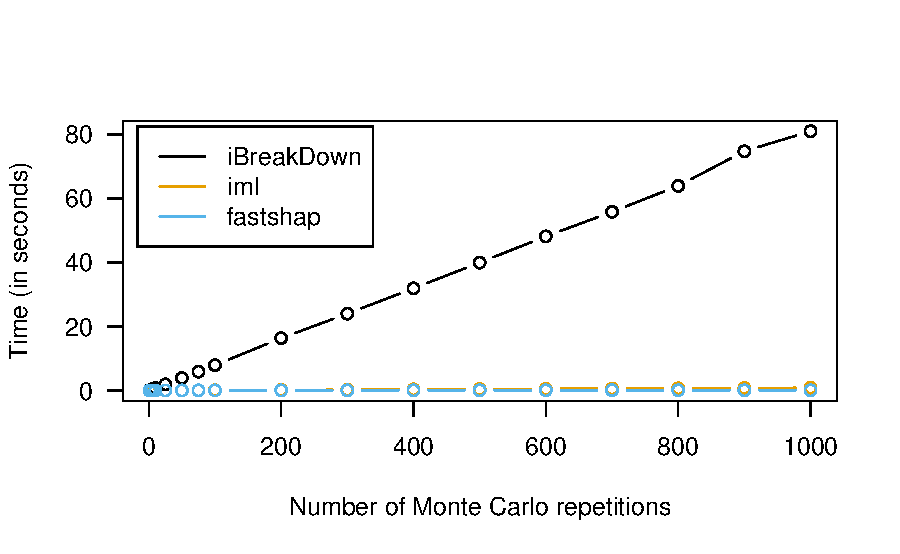
\includegraphics[width=1\linewidth]{greenwell_files/figure-latex/ex-titanic-benchmark-1}

In this example, for \(R = 1000\) MC repetitions, \pkg{fastshap} is roughly \texttt{8.0229885} times faster than \pkg{iml}, and nearly \texttt{579.6091954} times faster than \pkg{iBreakDown}.

\hypertarget{example-visualizing-global-explanations-with-and}{%
\section{\texorpdfstring{Example: visualizing global explanations with \pkg{fastshap} and \pkg{shapviz}}{Example: visualizing global explanations with  and }}\label{example-visualizing-global-explanations-with-and}}

\hypertarget{example-predictingexplaining-als-progression}{%
\section{Example: predicting/explaining ALS progression}\label{example-predictingexplaining-als-progression}}

In this example, we'll do something a bit more interesting. Rather than demonstrating the use of \texttt{fastshap} on an ordinary prediction task, let's use it to help explain the output from a probabilistic regression framework that's (currently) only available in Python. To illustrate, we'll look at a brief example using the ALS data from \citet[p.~349]{efron-2016-computer}. A description of the data, along with the original source and download instructions, can be found at \url{https://web.stanford.edu/~hastie/CASI/}\}.

The data concern \(N = 1,822\) observations on \emph{amyotrophic lateral sclerosis} (ALS or Lou Gehrig's disease) patients. The goal is to predict ALS progression over time, as measured by the slope (or derivative) of a functional rating score (\texttt{dFRS}), using 369 available predictors obtained from patient visits. The data were originally part of the DREAM-Phil Bowen ALS Predictions Prize4Life challenge. The winning solution (Küffner et al. 2015) used a tree-based ensemble quite similar to a \emph{random forest} (Breiman 2001), while Efron and Hastie (2016) (Chap. 17) analyzed the data using a \emph{gradient boosted tree ensemble} (Friedman 2001, 2002).

Many classification tasks are inherently probabilistic. For example, probability forests (Malley et al. 2012) can be used to obtain consistent probability estimates for the different class outcomes (i.e., \(Pr\left(y = j|\boldsymbol{x}\right)\)). Regression tasks, on the other hand, are typically not probabilistic and the predictions correspond to some location estimate of \(y|\boldsymbol{x}\); that is, the distribution of \(y\) conditional on a set of predictor values \(\boldsymbol{x}\). For instance, the terminal nodes in a regression tree---which are used to compute fitted values and predictions---provide an estimate of the conditional mean \(E\left(y|\boldsymbol{x}\right)\). Often, it is of scientific interest to know about the probability of specific events conditional on a set of features, rather than a single point estimate like \(E\left(y|\boldsymbol{x}\right)\). In the ALS example, rather than using an estimate of the conditional mean \(\hat{f}\left(\boldsymbol{x}\right) = \hat{E}\left(\texttt{dFRS}|\boldsymbol{x}\right)\) to predict ALS progression for a new patient, it might be more useful to estimate \(Pr\left(\texttt{dFRS} < c | \boldsymbol{x}\right)\), for some constant \(c\). This is where probabilistic regression/forecasting comes in.

Probabilistic regression models provide estimates of the entire probability distribution of the response conditional on a set of predictors, denoted \(\mathcal{D}_{\boldsymbol{\theta}}\left(y | \boldsymbol{x}\right)\), where \(\boldsymbol{\theta}\) represents the parameters of the conditional distribution. For example, the normal distribution has \(\boldsymbol{\theta} = \left(\mu, \sigma\right)\); examples include \emph{generalized additive models for shape, scale, and location} (GAMLSS) (Rigby and Stasinopoulos 2005), \emph{Bayesian additive regression trees} (BART) (Chipman, George, and McCulloch 2010), and Bayesian deep learning. While several approaches to probabilistic regression exist, many of them are inflexible (e.g., GAMSLSS), computationally expensive (e.g., BART), or inaccessible to non-experts (e.g., Bayesian deep learning) (Duan et al. 2020). \emph{Natural gradient boosting} (NGBoost) extends the simple ideas of gradient boosting to probabilistic regression by treating the parameters \(\boldsymbol{\theta}\) as targets for a multiparameter boosting algorithm similar to gradient boosting. We say ``multiparameter'' because NGBoost fits a separate model for each parameter at every iteration.

The ``natural'' in ``natural gradient boosting'' refers to the fact that NGBoost uses something called the \emph{natural gradient}, as opposed to the ordinary gradient. The natural gradient provides the direction of steepest descent in \emph{Riemannian space}; this is necessary since gradient descent in the parameter space is not gradient descent in the distribution space because distances don't correspond. The important thing to remember is that NGBoost approximates the gradient of a proper scoring rule---similar to a loss function, but for predicted probabilities and probability distributions of the observed data---as a function of \(\boldsymbol{\theta}\). Compared to alternative probabilistic regression methods, NGBoost is fast, flexible, scalable, and easy to use. NGBoost is available in the \texttt{ngboost} package for Python. For more info, check out the NGBoost GitHub repository at \url{https://github.com/stanfordmlgroup/ngboost}.

To start, we'll read in the data from the companion website to Efron and Hastie (2016). Note that the data already include an indicator for training and validation, so we'll go ahead and split the data into train/validation sets:

\begin{verbatim}
als <- read.table("https://web.stanford.edu/~hastie/CASI_files/DATA/ALS.txt", 
                  header = TRUE)

# Split into train/test sets
als.trn <- als[!als$testset, -1]  # train
als.val <- als[als$testset, -1]  # validation

# Print dimensions
dim(als.trn)
\end{verbatim}

\begin{verbatim}
#> [1] 1197  370
\end{verbatim}

\begin{verbatim}
dim(als.val)
\end{verbatim}

\begin{verbatim}
#> [1] 625 370
\end{verbatim}

Next, we'll use \CRANpkg{reticulate} (\textbf{FIXME:} need citation) to load the Python \texttt{ngboost} module:

\begin{verbatim}
library(reticulate)

ngboost <- import("ngboost")  # requires installation of ngboost

# Construct an NGBoost regressor object
ngb <- ngboost$NGBRegressor(
  Dist = ngboost$distns$Normal,
  n_estimators = 2000L,
  learning_rate = 0.01,
  verbose_eval = 0,
  random_state = 1601L
)
\end{verbatim}

In the next chunk, we call the \texttt{ngb} object's fit()` method to actually train the model (the validation set is used with early stopping to determine the optimal number of trees in the ensemble):

\begin{verbatim}
X.trn <- subset(als.trn, select = -dFRS)  # features only
X.val <- subset(als.val, select = -dFRS)  # features only

# Train the model
ngb$fit(
  X = X.trn,
  Y = als.trn$dFRS,
  X_val = X.val,
  Y_val = als.val$dFRS,
  early_stopping_rounds = 5L
)
\end{verbatim}

\begin{verbatim}
#> NGBRegressor(n_estimators=2000,
#>              random_state=RandomState(MT19937) at 0x7F5222D48040,
#>              verbose_eval=0.0)
\end{verbatim}

\begin{verbatim}
ngb$predict(X.val[1, ])
\end{verbatim}

\begin{verbatim}
#> [1] -0.4649206
\end{verbatim}

\begin{verbatim}
(params <- ngb$pred_dist(X.val[1, ])$params)
\end{verbatim}

\begin{verbatim}
#> $loc
#> [1] -0.4649206
#> 
#> $scale
#> [1] 0.4386185
\end{verbatim}

The code chunk below generates a plot of the estimated cumulative probability density function (i.e., \(Pr\left(\texttt{dFRS} <= t\right)\)) for the first observation in the validation set; see Figure \ref{fig:als-ngb-normal}.

\begin{verbatim}
plot(function(x) pnorm(x, mean = params$loc, sd = params$scale), 
     from = min(als$dFRS), to = max(als$dFRS),
     xlab = "dFRS", ylab = "Cumulative probability")
\end{verbatim}

\begin{figure}
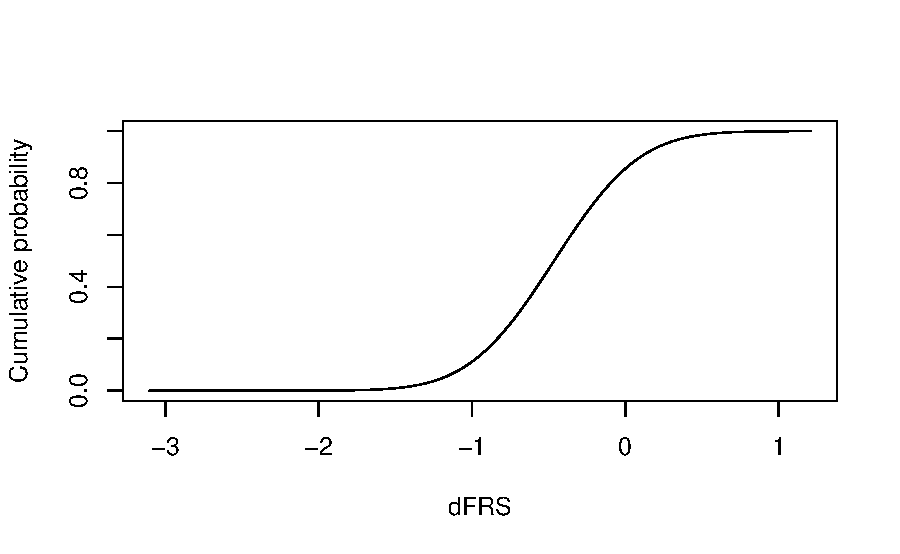
\includegraphics[width=1\linewidth]{greenwell_files/figure-latex/als-ngb-normal-1} \caption{ABC.}\label{fig:als-ngb-normal}
\end{figure}

Since \texttt{ngboost} is built on top of \texttt{sklearn} (Pedregosa et al. 2011), we can actually use the Python \texttt{shap} package (Scott M. Lundberg and Lee 2017a) to create efficient explanations for the model. Below, we call the \texttt{TreeExplainer()} method on the training set and generate global some global interpretations: a variable importance plot, and a \emph{SHAP dependence plot}:

\begin{verbatim}
library(ggplot2)
library(shapviz)

# Use 'shap' package to compute SHAP values for entire training set
shap <- import("shap")
explainer <- shap$TreeExplainer(ngb, model_output = 0L)
ex.trn <- explainer$shap_values(X.trn)  # training explanations
colnames(ex.trn) <- colnames(X.trn)

# Construct variable importance and SHAP dependence plots
viz <- shapviz(ex.trn, X = X.trn)
p1 <- sv_importance(viz) + theme_bw()
p2 <- sv_dependence(viz, v = "Onset.Delta", alpha = 0.3) + theme_bw()
gridExtra::grid.arrange(p1, p2, nrow = 1)
\end{verbatim}

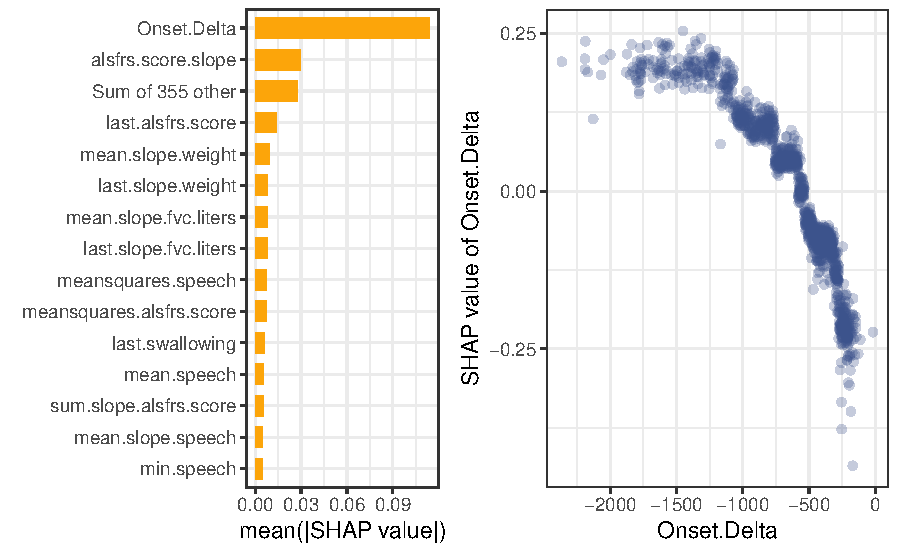
\includegraphics[width=1\linewidth]{greenwell_files/figure-latex/als-ngboost-shap-1}

A \texttt{dFRS} of less than -1.1 is considered to be fast progression (Küffner et al. 2015). Hence, it could be useful to estimate the probability of \texttt{dFRS\ \textless{}\ -1.1} and provide an explanation for any individual who's corresponding probability is considered high. The prediction wrapper (\texttt{pfun()}) defined below computes the cumulative probability \(Pr\left(\texttt{dFRS} < -1.1 | \boldsymbol{x}\right)\). We use it to determine the observation in the validation set with the highest cumulative probability:

\begin{verbatim}
pfun <- function(object, newdata) {
  dist <- object$pred_dist(newdata)
  pnorm(-1.1, mean = dist$params$loc, sd = dist$params$scale)
}

max(prob.val <- pfun(ngb, newdata = X.val))
\end{verbatim}

\begin{verbatim}
#> [1] 0.754336
\end{verbatim}

\begin{verbatim}
xval.max <- X.val[which.max(prob.val), ]  # obs with highest predicted prob
\end{verbatim}

\begin{verbatim}
library(fastshap)

system.time({
  set.seed(1110)
  ex <- explain(ngb, X = X.trn, nsim = 100, pred_wrapper = pfun, 
                newdata = xval.max, adjust = TRUE)
})
\end{verbatim}

\begin{verbatim}
#>    user  system elapsed 
#> 115.697   0.080 115.779
\end{verbatim}

\begin{verbatim}
# Visualize with a force plot
viz <- shapviz(ex, X = xval.max, baseline = attr(ex, which = "baseline"))
sv_waterfall(viz, max_display = 10)
\end{verbatim}

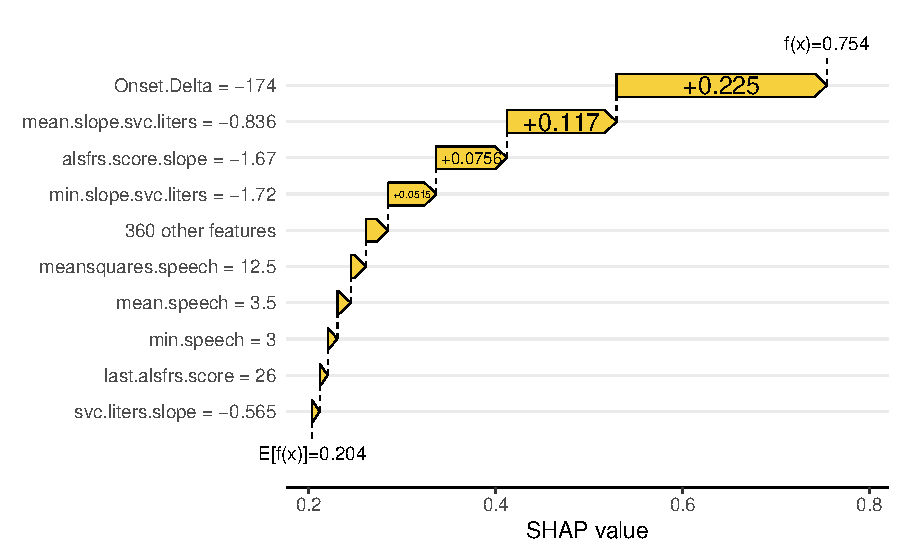
\includegraphics[width=1\linewidth]{greenwell_files/figure-latex/als-ngboost-fastshap-1}

\hypertarget{refs}{}
\begin{CSLReferences}{1}{0}
\leavevmode\vadjust pre{\hypertarget{ref-aas-2020-explaining}{}}%
Aas, Kjersti, Martin Jullum, and Anders Løland. 2020. {``Explaining Individual Predictions When Features Are Dependent: More Accurate Approximations to Shapley Values.''} \url{https://arxiv.org/abs/1903.10464}.

\leavevmode\vadjust pre{\hypertarget{ref-achen-1982-interpreting}{}}%
Achen, Christopher H. 1982. \emph{Interpreting and Using Regression}. Interpreting and Using Regression. Sage Publications.

\leavevmode\vadjust pre{\hypertarget{ref-R-iBreakDown}{}}%
Biecek, Przemyslaw, Alicja Gosiewska, Hubert Baniecki, and Adam Izdebski. 2020. \emph{iBreakDown: Model Agnostic Instance Level Variable Attributions}. \url{https://CRAN.R-project.org/package=iBreakDown}.

\leavevmode\vadjust pre{\hypertarget{ref-breiman-2001-rf}{}}%
Breiman, Leo. 2001. {``Random Forests.''} \emph{Machine Learning} 45 (1): 5--32. \url{https://doi.org/10.1023/A:1010933404324}.

\leavevmode\vadjust pre{\hypertarget{ref-R-R6}{}}%
Chang, Winston. 2021. \emph{R6: Encapsulated Classes with Reference Semantics}. \url{https://CRAN.R-project.org/package=R6}.

\leavevmode\vadjust pre{\hypertarget{ref-charnes-1988-extremal}{}}%
Charnes, A., B. Golany, M. Keane, and J. Rousseau. 1988. {``Extremal Principle Solutions of Games in Characteristic Function Form: Core, Chebychev and Shapley Value Generalizations.''} In \emph{Econometrics of Planning and Efficiency}, edited by Jati K. Sengupta and Gopal K. Kadekodi, 123--33. Dordrecht: Springer Netherlands. \url{https://doi.org/10.1007/978-94-009-3677-5_7}.

\leavevmode\vadjust pre{\hypertarget{ref-chen-2020-true}{}}%
Chen, Hugh, Joseph D. Janizek, Scott Lundberg, and Su-In Lee. 2020. {``True to the Model or True to the Data?''} \url{https://arxiv.org/abs/2006.16234}.

\leavevmode\vadjust pre{\hypertarget{ref-R-xgboost}{}}%
Chen, Tianqi, Tong He, Michael Benesty, Vadim Khotilovich, Yuan Tang, Hyunsu Cho, Kailong Chen, et al. 2020. \emph{Xgboost: Extreme Gradient Boosting}. \url{https://github.com/dmlc/xgboost}.

\leavevmode\vadjust pre{\hypertarget{ref-chipman-2010-bart}{}}%
Chipman, Hugh A., Edward I. George, and Robert E. McCulloch. 2010. {``{BART: Bayesian additive regression trees}.''} \emph{The Annals of Applied Statistics} 4 (1): 266--98. \url{https://doi.org/10.1214/09-AOAS285}.

\leavevmode\vadjust pre{\hypertarget{ref-covert-2021-improving}{}}%
Covert, Ian, and Su-In Lee. 2021. {``Improving KernelSHAP: Practical Shapley Value Estimation via Linear Regression.''} \url{https://arxiv.org/abs/2012.01536}.

\leavevmode\vadjust pre{\hypertarget{ref-R-pkgsearch}{}}%
Csárdi, Gábor, and Maëlle Salmon. 2020. \emph{Pkgsearch: Search and Query CRAN r Packages}. \url{https://CRAN.R-project.org/package=pkgsearch}.

\leavevmode\vadjust pre{\hypertarget{ref-duan-2020-ngboost}{}}%
Duan, Tony, Anand Avati, Daisy Yi Ding, Khanh K. Thai, Sanjay Basu, Andrew Y. Ng, and Alejandro Schuler. 2020. {``NGBoost: Natural Gradient Boosting for Probabilistic Prediction.''} arXiv. \url{https://doi.org/10.48550/ARXIV.1910.03225}.

\leavevmode\vadjust pre{\hypertarget{ref-efron-2016-computer}{}}%
Efron, Bradley, and Trevor Hastie. 2016. \emph{Computer Age Statistical Inference: Algorithms, Evidence, and Data Science}. Institute of Mathematical Statistics Monographs. Cambridge University Press. \url{https://doi.org/10.1017/CBO9781316576533}.

\leavevmode\vadjust pre{\hypertarget{ref-friedman-2001-greedy}{}}%
Friedman, Jerome H. 2001. {``Greedy Function Approximation: A Gradient Boosting Machine.''} \emph{The Annals of Statistics} 29 (5): 1189--1232. \url{https://doi.org/10.1214/aos/1013203451}.

\leavevmode\vadjust pre{\hypertarget{ref-friedman-2002-stochastic}{}}%
---------. 2002. {``Stochastic Gradient Boosting.''} \emph{Computational Statistics \& Data Analysis} 38 (4): 367--78. https://doi.org/\url{https://doi.org/10.1016/S0167-9473(01)00065-2}.

\leavevmode\vadjust pre{\hypertarget{ref-gosiewska-2019-iBreakDown}{}}%
Gosiewska, Alicja, and Przemyslaw Biecek. 2019. {``iBreakDown: Uncertainty of Model Explanations for Non-Additive Predictive Models.''} \emph{CoRR} abs/1903.11420. \url{http://arxiv.org/abs/1903.11420}.

\leavevmode\vadjust pre{\hypertarget{ref-R-fastshap}{}}%
Greenwell, Brandon. 2020. \emph{Fastshap: Fast Approximate Shapley Values}. \url{https://github.com/bgreenwell/fastshap}.

\leavevmode\vadjust pre{\hypertarget{ref-kuffner-2015-als}{}}%
Küffner, Robert, Neta Zach, Raquel Norel, Johann Hawe, David Schoenfeld, Liuxia Wang, Guang Li, et al. 2015. {``Crowdsourced Analysis of Clinical Trial Data to Predict Amyotrophic Lateral Sclerosis Progression.''} \emph{Nature Biotechnology} 33 (1): 51--57. \url{https://doi.org/10.1038/nbt.3051}.

\leavevmode\vadjust pre{\hypertarget{ref-lundberg-2020-treeshap}{}}%
Lundberg, Scott M., Gabriel Erion, Hugh Chen, Alex DeGrave, Jordan M. Prutkin, Bala Nair, Ronit Katz, Jonathan Himmelfarb, Nisha Bansal, and Su-In Lee. 2020. {``From Local Explanations to Global Understanding with Explainable AI for Trees.''} \emph{Nature Machine Intelligence} 2 (1): 2522--5839.

\leavevmode\vadjust pre{\hypertarget{ref-lundberg-2017-shap}{}}%
Lundberg, Scott M., and Su-In Lee. 2017a. {``A Unified Approach to Interpreting Model Predictions.''} In \emph{Advances in Neural Information Processing Systems 30}, edited by I. Guyon, U. V. Luxburg, S. Bengio, H. Wallach, R. Fergus, S. Vishwanathan, and R. Garnett, 4765--74. Curran Associates, Inc. \url{http://papers.nips.cc/paper/7062-a-unified-approach-to-interpreting-model-predictions.pdf}.

\leavevmode\vadjust pre{\hypertarget{ref-lundberg-2017-KernelSHAP}{}}%
Lundberg, Scott M, and Su-In Lee. 2017b. {``A Unified Approach to Interpreting Model Predictions.''} In \emph{Advances in Neural Information Processing Systems 30}, edited by I. Guyon, U. V. Luxburg, S. Bengio, H. Wallach, R. Fergus, S. Vishwanathan, and R. Garnett, 4765--74. Curran Associates, Inc. \url{http://papers.nips.cc/paper/7062-a-unified-approach-to-interpreting-model-predictions.pdf}.

\leavevmode\vadjust pre{\hypertarget{ref-malley-2012-consistent}{}}%
Malley, James D., Jochen Kruppa, Abhijit Dasgupta, Karen Godlove Malley, and Andreas Ziegler. 2012. {``Probability Machines: Consistent Probability Estimation Using Nonparametric Learning Machines.''} \emph{Methods of Information in Medicine} 51 (1): 74--81. \url{https://doi.org/10.3414/ME00-01-0052}.

\leavevmode\vadjust pre{\hypertarget{ref-R-shapviz}{}}%
Mayer, Michael. 2022. \emph{Shapviz: SHAP Visualizations}. \url{https://CRAN.R-project.org/package=shapviz}.

\leavevmode\vadjust pre{\hypertarget{ref-molnar-2019-iml}{}}%
Molnar, Christoph. 2019. \emph{Interpretable Machine Learning: A Guide for Making Black Box Models Explainable}.

\leavevmode\vadjust pre{\hypertarget{ref-R-iml}{}}%
Molnar, Christoph, and Patrick Schratz. 2020. \emph{Iml: Interpretable Machine Learning}. \url{https://CRAN.R-project.org/package=iml}.

\leavevmode\vadjust pre{\hypertarget{ref-pearl-2009-causality}{}}%
Pearl, Judea. 2009. \emph{Causality: Models, Reasoning and Inference}. 2nd ed. USA: Cambridge University Press.

\leavevmode\vadjust pre{\hypertarget{ref-scikit-learn}{}}%
Pedregosa, F., G. Varoquaux, A. Gramfort, V. Michel, B. Thirion, O. Grisel, M. Blondel, et al. 2011. {``Scikit-Learn: Machine Learning in {P}ython.''} \emph{Journal of Machine Learning Research} 12: 2825--30.

\leavevmode\vadjust pre{\hypertarget{ref-rigby-2005-gamlss}{}}%
Rigby, Robert A., and Mikis D. Stasinopoulos. 2005. {``Generalized Additive Models for Location, Scale and Shape.''} \emph{Journal of the Royal Statistical Society: Series C (Applied Statistics)} 54 (3): 507--54. https://doi.org/\url{https://doi.org/10.1111/j.1467-9876.2005.00510.x}.

\leavevmode\vadjust pre{\hypertarget{ref-shapley-2016-value}{}}%
Shapley, Lloyd S. 2016. {``17. A Value for n-Person Games.''} In \emph{Contributions to the Theory of Games (AM-28), Volume II}, edited by Harold William Kuhn and Albert William Tucker, 307--18. Princeton University Press. \url{https://doi.org/10.1515/9781400881970-018}.

\leavevmode\vadjust pre{\hypertarget{ref-R-lightgbm}{}}%
Shi, Yu, Guolin Ke, Damien Soukhavong, James Lamb, Qi Meng, Thomas Finley, Taifeng Wang, et al. 2022. \emph{Lightgbm: Light Gradient Boosting Machine}. \url{https://CRAN.R-project.org/package=lightgbm}.

\leavevmode\vadjust pre{\hypertarget{ref-strumbelj-2014-explaining}{}}%
Štrumbelj, Erik, and Igor Kononenko. 2014. {``Explaining Prediction Models and Individual Predictions with Feature Contributions.''} \emph{Knowledge and Information Systems} 31 (3): 647--65. \url{https://doi.org/10.1007/s10115-013-0679-x}.

\leavevmode\vadjust pre{\hypertarget{ref-zhao-2021-causal}{}}%
Zhao, Qingyuan, and Trevor Hastie. 2021. {``Causal Interpretations of Black-Box Models.''} \emph{Journal of Business \& Economic Statistics} 39 (1): 272--81. \url{https://doi.org/10.1080/07350015.2019.1624293}.

\end{CSLReferences}

\bibliography{greenwell.bib}

\address{%
Brandon M. Greenwell\\
University of Cincinnati\\%
2925 Campus Green Dr\\ Cincinnati, OH 45221\\ United States of America\\
%
\url{https://github.com/bgreenwell}\\%
\textit{ORCiD: \href{https://orcid.org/0000-0002-8120-0084}{0000-0002-8120-0084}}\\%
\href{mailto:greenwell.brandon@gmail.com}{\nolinkurl{greenwell.brandon@gmail.com}}%
}
